\documentclass[11pt]{article}
\usepackage[utf8]{inputenc} % Para caracteres en espa�ol
\usepackage{amsmath,amsthm,amsfonts,amssymb,amscd}
\usepackage{multirow,booktabs}
\usepackage[table]{xcolor}
\usepackage{fullpage}
\usepackage{lastpage}
\usepackage{enumitem}
\usepackage{multicol}
\usepackage{fancyhdr}
\usepackage{mathrsfs}
\usepackage{wrapfig}
\usepackage{setspace}
\usepackage{esvect}
\usepackage{calc}
\usepackage{multicol}
\usepackage{cancel}
\usepackage{graphicx}
\graphicspath{ {pictures/} }
\usepackage[retainorgcmds]{IEEEtrantools}
\usepackage[margin=3cm]{geometry}
\usepackage{amsmath}
\newlength{\tabcont}
\setlength{\parindent}{0.0in}
\setlength{\parskip}{0.05in}
\usepackage{empheq}
\usepackage{framed}
\usepackage[most]{tcolorbox}
\usepackage{xcolor}
\colorlet{shadecolor}{orange!15}
\parindent 0in
\parskip 12pt
\geometry{margin=1in, headsep=0.25in}
\theoremstyle{definition}
\newtheorem{defn}{Definition}
\newtheorem{reg}{Rule}
\newtheorem{exer}{Exercise}
\newtheorem{note}{Note}
\newcommand{\volume}{{\ooalign{\hfil$V$\hfil\cr\kern0.08em--\hfil\cr}}}
\newcommand{\parr}{\mathbin{\|}} % Parralel Symbol
\begin{document}
\setcounter{section}{0}
 \pagestyle{fancy}
\fancyhf{}
\rhead{Section 2: Electromagnetics}
\rfoot{Page \thepage}
\thispagestyle{empty}
\begin{center}
{\LARGE \bf Section 2: Electromagnetics}\\
{\large AE435}\\
Spring 2018
\end{center}
In this section, we will review the basics of charge, electricity, magnetism, and Maxwell equations.
\vspace{25mm}
\section{Electrostatics}
\vspace{5mm}
\tableofcontents
\newpage
\subsection{Coulomb's Law}
Coulomb's Law is the measure of force between charges. 
\newline
\newline
\newline
\textbf{Case 1: Two Particles}
\newline
\newline
Consider two charges $q_2$ and $q_2$ located at $\vv{r_1}$ and $\vv{r_2}$.
\begin{center}
\vspace{40mm}
\textbf{Figure 1}
\end{center}
The force on $q_1$ due to $q_2$ is
\begin{shaded}
\textbf{Coulomb Force} \newline
\begin{equation}
\vv{F_{12}} = c (\frac{q_1 q_2}{r_{12}^{2}}) \frac{\vv{r_{12}}}{r_{12}} \quad \sim \quad \frac{1}{r^2}
\end{equation}
Where:
\begin{equation*}
\begin{split}
\vv{r_{12}} = \vv{r_1}-\vv{r_2} \qquad &\text{The Sum of Position Vectors} \\
r_{12} = \lvert \vv{r_{12}} \rvert \qquad &\text{The Magnitude of $\vv{r_{12}}$} \\ \\
c = \qquad & \text{Coulomb's Constant} \\
 & = \quad 8.9875x10^9 = \frac{1}{4\pi \epsilon_0} [\frac{N m^2}{c^2}] \\ \\
\epsilon_{0} =  \qquad & \text{Permittivity of Free Space} \\
& = \quad 8.854x10^{-12} [\frac{c^2}{N m^2}]
\end{split}
\end{equation*}
\end{shaded}
Coulomb force scales with the square of the distance as shown by $\sim \frac{1}{r^2}$ in Equation 1.
\newpage
\textbf{Case 2: Many Particles - Coulomb Law}
\newline
\begin{defn} \textbf{Principle of superposition: } \\
Attraction between any pair can be calculated with Equation 1, regardless of the number of particles in the ensemble.
\end{defn}
So, let $\vv{r_i}$ be location of test particle $q_i$. If we have N charged particles, the force on $q_i$ is the linear superposition of the individual forces,
\begin{shaded}
\textbf{Multiple Particle Coulomb Force} \newline
\begin{equation}
\vv{F_{ij}} = \frac{q_i}{4\pi \epsilon_0} \sum_{j \neq i}^{N} q_i \bigg(\frac{\vv{r_{ij}}}{r_{ij}^3}\bigg)
\end{equation}
Where:
\begin{equation*}
\begin{split}
\vv{r_{ij}} = \vv{r_i}-\vv{r_j} \qquad &\text{The vector from test particle $q_i$ to field particle $q_j$} \\
\end{split}
\end{equation*}
\end{shaded}
\newline
\textbf{Case 3: Continuum Generalizations}
\newline \newline
Let us define
\begin{itemize}
\item \textbf{Volume Charge Density} $[\frac{C}{m^3}]$
\begin{equation}
\begin{aligned}
\rho_{e} = \lim_{\Delta \volume \rightarrow 0} \frac{\Delta q}{\Delta \volume}
\end{aligned}
\end{equation}
\item \textbf{Surface Charge Density} $[\frac{C}{m^2}]$
\begin{equation}
\begin{aligned}
\sigma_{e} = \lim_{\Delta \text{S} \rightarrow 0} \frac{\Delta q}{\Delta S}
\end{aligned}
\end{equation}
\end{itemize}
With these, the force acting on charge $q_o$ due to distributed charge sources are:
\begin{shaded}
\textbf{Continuum Charge Coulomb Force} \newline
\begin{equation}
\vv{F_{q_o}} = \frac{q_i}{4\pi \epsilon_0} \Bigg[ \int_{\volume} \frac{\vv{r}-\vv{r}'}{|\vv{r}-\vv{r}'|^3}\rho_{e}(\vv{r}')\mathrm{d}\vv{\volume} + \int_{S}  \frac{\vv{r}-\vv{r}'}{|\vv{r}-\vv{r}'|^3}\sigma_{e}(\vv{r}')\mathrm{d}\vv{S}\Bigg]
\end{equation}
Where:
\begin{equation*}
\begin{split}
\vv{r}' =& \text{ The location within $\volume$ or location on S} \\
\vv{r} =& \text{ The location of $q_o$} \\
\sigma_{e} \text{ and } \rho_{e} =&  \text{ Functions of position $\vv{r}'$} \\
\end{split}
\end{equation*}
\end{shaded}
\newpage
\subsection{Electric Field}
\begin{framed}
\begin{equation}
\vv{E} = \lim_{q_0 \rightarrow 0} \frac{F_{q_o}}{q_o}
\end{equation}
\end{framed}
The force acting on a specific charge $q_o$ from a collection of other charges per unit charge, as the specific charge tends to zero.
\newline
\newline
We set $q_0 \rightarrow 0$ so its presence does not influence the ambient charge.
\newline
\newline
Adding Equation 2 and Equation 5 then dividing thru by q results in:
\begin{shaded}
\textbf{Electric Field Equation} \newline
\begin{equation}
\vv{E} = \frac{q_i}{4\pi \epsilon_0} \Bigg[ \sum_{i=1}^{N} q \frac{\vv{r}-\vv{r_i}}{|\vv{r}-\vv{r_i}|^3} + \int_{\volume} \frac{\vv{r}-\vv{r}'}{|\vv{r}-\vv{r}'|^3}\rho_{e}(\vv{r}')\mathrm{d}\vv{\volume} + \int_{S}  \frac{\vv{r}-\vv{r}'}{|\vv{r}-\vv{r}'|^3}\sigma_{e}(\vv{r}')\mathrm{d}\vv{S}\Bigg]
\end{equation}
Where:
\begin{equation*}
\begin{split}
\vv{E} =& \vv{E}(\vv{r}) \quad \text{ Electric Field is a function of position $\vv{r}$} \\
\end{split}
\end{equation*}
\end{shaded}
We can use integral approach to solve problems, but this can get complex. We can also visualize the Electric Field via field lines, curves that are everywhere tangent to the field.
\newline
\begin{center}
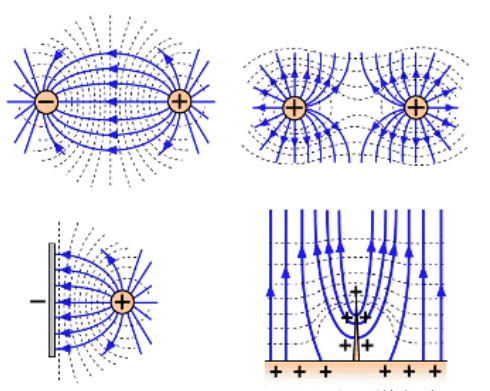
\includegraphics[scale=0.5]{1.png}
\end{center}
\newpage
\subsection{Conductors and Insulators}
\begin{defn} \textbf{Conductor:} Free charges, respond to external Electric field
with charge motion.\end{defn}
\begin{defn} \textbf{Insulator:} Bound charges, no motion. Also often called a
"dielectric"\end{defn}
\subsection{Gauss's Law}
\newline
\begin{defn} \textbf{Gauss's Law:}  Relates the electric field at a surface to the charge enclosed within that surface. The total flux that passes through any closed surface is proportional to the electric charge enclosed by a surface. This surface is the Gaussian Surface.\end{defn}
\textbf{Case 1: Single Charge}
\newline
\newline
The electric field for a single charge is
\begin{framed}
\begin{equation}
\vv{E} = \frac{q}{4\pi \epsilon_0} \frac{\vv{r}}{r^3}
\end{equation}
\end{framed}
If we take the surface integral around an arbitrary volume surrounding the charge we get:
\begin{center}
\vfill
\textbf{Figure 2}
\end{center}
\begin{shaded}
\textbf{Gauss' Law for Electric Fields} \newline
\begin{equation}
\oint_{S} \vv{E}\cdot \hat{n} \, \mathrm{d}A = \frac{q}{4 \pi \epsilon_0} \oint_{S} \frac{\vv{r} \cdot \hat{n}}{r^3} \, \mathrm{d}A
\end{equation}
Where:
\begin{equation*}
\begin{split}
\bigg( \frac{\vv{r}}{r} \bigg) \cdot \hat{n} \, \mathrm{d}A  &= \text{The project of dA on a plane perpendicular to $\vv{r}$} \\
\end{split}
\end{equation*}
\end{shaded}
\newpage
If we divide the projected area, $\bigg( \frac{\vv{r}}{r} \bigg) \cdot \hat{n} \, \mathrm{d}A$, by $r^2$, we arrive at the solid angle $\mathrm{d}\Omega$.
\begin{center}
\vfill
\textbf{Figure 3}
\end{center}
The total solid angle subtended by a surface totally enclosing the charge is $4 \pi$, so 
\begin{equation*}
\oint_{S} \frac{\vv{r} \cdot \hat{n}}{r^3} \, \mathrm{d}A = 4 \pi 
\end{equation*}
As a result, Equation 9 becomes:
\begin{framed}
\begin{equation}
\oint_{S} \vv{E}\cdot \hat{n} \, \mathrm{d}A = \frac{q}{\epsilon_0} 
\end{equation}
\end{framed}
\textbf{Case 2: Many Point Charges}
\newline
\newline
For the case of many point charges, we take the sum:
\begin{equation*}
\oint_{S} \vv{E}\cdot \hat{n} \, \mathrm{d}A = \frac{1}{\epsilon_0} \sum_{i = 1}^{N} qi
\end{equation*}
\textbf{Case 3: Distributed Charge}
\newline
\newline
For a distributed charge, $\rho_e$, we take the integral over the enclosed volume:
\begin{shaded}
\textbf{Integral Form of Gauss's Law} \newline
\begin{equation}
\oint_{S} \vv{E}\cdot \hat{n} \, \mathrm{d}A = \frac{1}{\epsilon_0} \int_{\volume} \rho_e \, \mathrm{d}\volume
\end{equation}
\end{shaded}
\newpage
Also recall Divergence Theorem (also known as Gauss's Theorem):
\begin{shaded}
\textbf{Divergence Theroem} \newline
\begin{equation}
\oint_{S} \vv{F}\cdot \hat{n} \, \mathrm{d}A = \int_{\volume} \nabla \cdot \vv{F} \, \mathrm{d}\volume
\end{equation}
\end{shaded}
which applies to any vector field $\vv{F}$, so we arrive that...
\begin{equation*}
\oint_{S} \vv{E}\cdot \hat{n} \, \mathrm{d}A = \int_{\volume} \nabla \cdot \vv{E} \mathrm{d}\volume = \frac{1}{\epsilon_0} \int_{\volume} \rho_e \, \mathrm{d}\volume
\end{equation*}
\begin{shaded}
\textbf{Differential Form of Gauss's Law} \newline
\begin{equation}
\nabla \cdot \vv{E} = \frac{1}{\epsilon_0} \rho_{e}
\end{equation}
\end{shaded}
\newpage
\subsection{Electrostatic Potential and Energy}
One can show that the curl of the electric field is zero for an electrostatic field. 
\newline
In general $\nabla \times \vv{E} = -\frac{\partial \vv{B}}{\partial t} = 0$ as we will see later.
\begin{equation}
\nabla \times \vv{E} = 0
\end{equation}
We also use the vector identity:
\begin{equation}
\nabla \times \nabla \phi = 0
\end{equation}
\newline
From Equation 14 and Equation 15, we can see the relation $\vv{E}=\nabla \phi$, such that the vector field $\vv{E}$ is related to the gradient in some scalar field.
\newline
\newline
We call $\phi$ the \textbf{electric potential}. And actually use
\newline
\begin{equation}
\vv{E} = - \nabla \phi(\vv{r})
\end{equation}
\newline
For a single point charge $q_i$ at $\vv{r_i}$, by integrating Equation 16, we arrive at:
\newline
\begin{equation*}
\phi(\vv{r}) = \frac{1}{4 \pi \epsilon_0} \frac{q_1}{|\vv{r}-\vv{r_1}|}+\text{constant}
\end{equation*}
\newline
On any curve linking point $P_1$ to point $P_2$ ,
\newline
\begin{equation*}
\phi_{12} (\vv{r}) = \int_{P_i}^{P_2} \nabla \phi (\vv{r}) \cdot \mathrm{d}\vv{l} = - \int_{P_i}^{P_2} \vv{E}(\vv{r}) \cdot \mathrm{d}\vv{l}
\end{equation*}
\newline
Which tells us the work per unit charge to move from $P_1$ to $P_2$.
\newline
More generally,
\newline
\begin{equation*}
\phi(\vv{r}) = \frac{1}{4 \pi \epsilon_0} \Bigg[ \sum_{i=1}^{N} \frac{q_i}{|\vv{r}-\vv{r_i}|} + \int_{\volume} \frac{\rho_e (\vv{r})}{|\vv{r}-\vv{r}'|} \, \mathrm{d}\vv{\volume} + \int_{S}  \frac{\sigma_{e}(\vv{r})}{|\vv{r}-\vv{r}'|} \, \mathrm{d}A'\Bigg]+\text{constant}
\end{equation*}
\newline
Taking line integral from some reference location to $\vv{r}$,
\newline
\begin{equation*}
\int_{\text{ref}}^{\vv{r}} \vv{E}(\vv{r}) \cdot \mathrm{d}\vv{r} = - \int_{\text{ref}}^{\vv{r}} \nabla \phi(\vv{r}) \cdot \mathrm{d}\vv{r} = - \int_{\text{ref}}^{\vv{r}} \mathrm{d}\phi = - \phi (\vv{r})- \phi_{ref}
\end{equation*}
\newline
Now if we set $\phi_{ref} = 0$ at $r \rightarrow \infty$. Then
\newline
\begin{equation}
\phi (\vv{r}) = -\int_{\text{ref}}^{\vv{r}} \vv{E}(\vv{r}) \cdot \mathrm{d}\vv{r}
\end{equation}
\newline
The Potential Energy, $U$, associated with a force $\vv{F}$ is
\newline
\begin{equation*}
U (\vv{r}) = -\int_{\text{ref}}^{\vv{r}} \vv{F}(\vv{r}) \cdot \mathrm{d}\vv{r}
\end{equation*}
\newline
Since $\vv{F} = q \vv{E}$ for electrostatic force as seen in Equation 16, the electrostatic potential is
\newline
\begin{shaded}
\textbf{Electrostatic Potential} \newline
\begin{equation}
\phi (\vv{r}) = \frac{U (\vv{r}) }{q}
\end{equation}
\newline
The electrostatic potential defines the potential energy per unit charge.
\end{shaded}
\newline
If we define $\phi (\infty) = 0$ then $U (\vv{r}) $ is the energy required to bring a test charge from $\vv{r} = \infty$ to $\vv{r}$.
\newpage
\subsection{Poisson and Laplace Equations}
For a charge distribution $q (\vv{r})$:
\newline
\begin{equation}
\phi(\vv{r}) = \frac{1}{4 \pi \epsilon_0} \int \frac{\partial q}{|\vv{r}-\vv{r}'|}
\end{equation}
\newline
Such that
\newline
\begin{equation}
\vv{E}(\vv{r}) =  \frac{1}{4 \pi \epsilon_0} \int \frac{(\vv{r}-\vv{r}') \, \mathrm{d} q}{|\vv{r}-\vv{r}'|^3}
\end{equation}
\newline
\newline
Since $\vv{E} = -\nabla \phi$ from Equation 16. We can solve for $\phi(\vv{r})$ and $\vv{E}(\vv{r})$ if we know $q(\vv{r})$ charge distribution. Alternatively, we can start with the differential form of Gauss's law (Equation 13) and Equation 16,
\newline
\begin{equation*}
\begin{align}
\nabla \cdot \vv{E} = \frac{\rho_e}{\epsilon_o} \qquad &\text{and} \qquad \vv{E} = - \nabla \phi \\ \\
\nabla \cdot (- \nabla & \phi) = \frac{\rho_e}{\epsilon_o} \\ \\
\text{Use laplacian: }& \nabla^2 = \nabla \cdot \nabla \rightarrow 
\end{align}
\end{equation*}
\begin{shaded}
\textbf{Poisson Equation} \newline
\begin{equation}
\nabla^2 \phi = -\frac{\rho_e}{\epsilon_o}
\end{equation}
Where:
\begin{equation*}
\begin{split}
\rho_e &= \rho_e (\vv{r}) \qquad \text{charge density distribution} \\
\phi &= \phi (\vv{r})  \qquad \text{electric potential distribution} \\
\end{split}
\end{equation*}
The Poisson Equation relates charge density distribution $\rho_e (\vv{r})$ to electric potential $\phi (\vv{r})$ distribution.
\end{shaded}
\newline
Alternatively,
\begin{shaded}
\textbf{Laplace Equation} \newline
\begin{equation}
\nabla^2 \phi = 0
\end{equation}
For region with no free (space) charge $\rho_e = 0$
\end{shaded}
\end{document}